\section{Experiments}
\label{sec:experiments}

\subsection{Setup}

We evaluate the framework on CPU and GPU traces collected from older GPT-style models and newer 4-bit instruct families. The strongest modern-family evidence comes from dense context sweeps on \texttt{Qwen2.5-1.5B}, \texttt{Qwen3-8B}, and \texttt{SmolLM2-1.7B}, together with an additional \texttt{Phi-3.5-mini} validation. Across the current artifact set, the main analysis covers 30 workload points. We report speedup relative to GPU-only execution under the virtual backend. Our primary realistic baselines are \texttt{online\_predictor}, \texttt{adaptive\_feature}, and \texttt{kv\_regime}; \texttt{oracle} serves only as an upper bound.

\subsection{Backend Transparency and Sensitivity}

The largest methodological risk in this paper is over-interpreting a virtual backend. We therefore make the backend explicit. \Cref{tab:backend-measured-modeled} separates trace-measured, trace-derived, and modeled quantities, while \Cref{tab:backend-params} lists the default parameters used by the virtual replay model. The most important anchor is that measured trace latency is used directly as the GPU reference whenever available; the roofline terms are then used only to decompose that measured latency into compute- and memory-dominant shares before applying the virtual PIM rescaling.

The sensitivity analysis is defensive but important. Conservative, default, and optimistic virtual-PIM presets change absolute speedups, but the canonical weak cases remain weak and the canonical long-context positive cases remain positive. We therefore treat the backend as a transparent what-if model whose main value lies in preserving regime ordering and relative decision-signal comparisons rather than exact numerical speedup claims.

\subsection{Negative Results Matter}

A key result of this study is that virtual PIM value is not automatic. \Cref{fig:negative-cases} shows this as a distribution rather than as a handful of cherry-picked bars. The left panel shows a clear mass of workloads near $\online = 1.0\times$, while the right panel shows that only $3/9$ short-context workloads are online-positive. The fraction rises to $9/9$ for mid-context workloads and $12/12$ for long-context workloads.

These negative results are important because they improve credibility. Rather than showing gains everywhere, the framework separates weak and positive regimes at the workload-distribution level, which makes the later positive-regime evidence more trustworthy. This also clarifies the main scientific claim: virtual PIM offload becomes interesting only after the decode stream enters the right operating regime, and short-context execution often fails to provide that signal.

\begin{figure}[t]
    \centering
    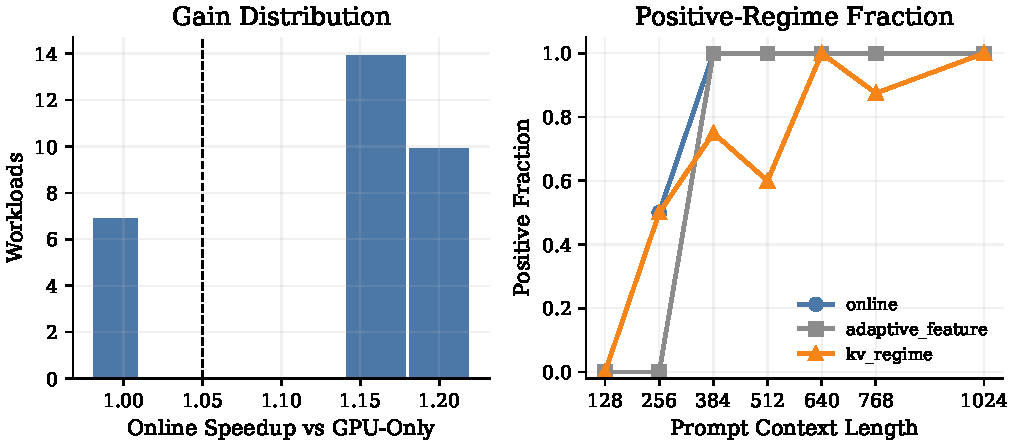
\includegraphics[width=0.95\linewidth]{figures/final_figures/paper_negative_cases.pdf}
    \caption{Distributional negative-result evidence. Left: workload-level distribution of realistic online gains. Right: positive-regime fraction versus context. Gains do not appear automatically, and short-context workloads are much more often weak.}
    \label{fig:negative-cases}
\end{figure}

\subsection{Context Governs Regime Entry}

\Cref{fig:context-transition} is the best-supported empirical result in the paper. It sharpens the regime transition using dense context sweeps instead of only coarse points such as 256, 512, and 768. The delayed-onset \texttt{Qwen2.5-1.5B} family transitions from weak to positive between 256 and 384 tokens, while \texttt{Qwen3-8B} and \texttt{SmolLM2-1.7B} become positive earlier, between 128 and 256 tokens. The extra \texttt{Phi-3.5-mini} validation remains positive at 256, 384, and 768 tokens, which shows that early-positive behavior is not isolated to a single family.

This result matters for two reasons. First, it supports a stronger claim than ``longer context helps'': in our current setup, context length is the clearest \emph{coarse} regime-entry variable. Second, it shows that onset is family-dependent rather than universal, which implies that a global rule such as ``offload attention after context 512'' is too coarse.

\subsection{KV-Related Signals Are Predictive, Not Causal}

\begin{figure}[t]
    \centering
    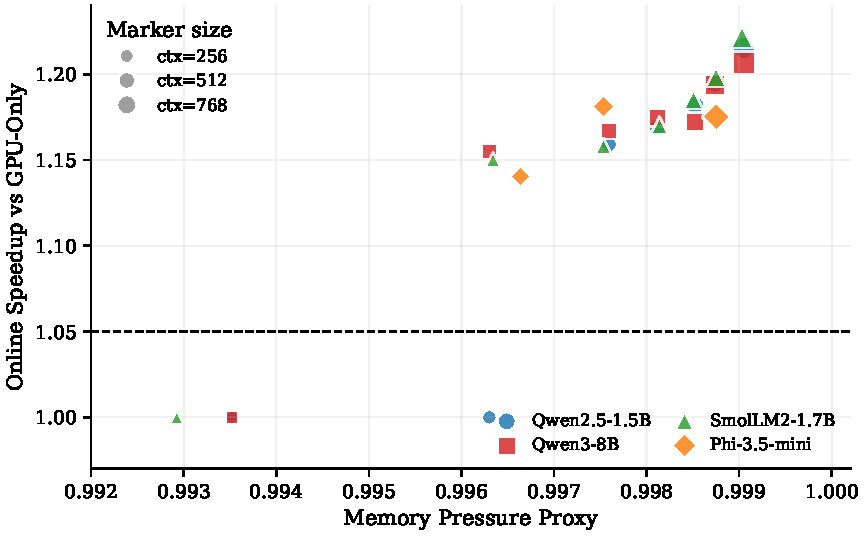
\includegraphics[width=0.95\linewidth]{figures/final_figures/paper_backbone_kv_pressure_vs_speedup.pdf}
    \caption{Higher memory-pressure proxy values align with positive online speedup across modern families. The figure is consistent with a KV-centered mechanism, but should be interpreted as predictive evidence rather than as causal proof.}
    \label{fig:kv-pressure}
\end{figure}

The mechanism analysis strengthens the paper beyond a context-only observation, but we intentionally stop short of a causal claim. Across the focused GPU suite, higher memory-pressure proxy values align with positive online speedup more directly than attention share alone. We therefore interpret the evidence as follows: the observed regime boundary is consistent with rising KV-cache-related pressure, and KV-related proxies are useful predictive correlates under the current backend.

This view also helps account for family-dependent onset. Different families can exhibit different KV-cache traffic profiles and attention behavior under similar context lengths, which means the same context value need not imply the same offload regime boundary.

\subsection{Held-Out Decision-Signal Study}

To test signal quality more directly, we built a workload-level classifier for positive-regime detection, where the label is whether the realistic online predictor reaches $\mathrm{speedup} > 1.05\times$. We compare five signal families: attention-only, context-only, context+attention, KV-only, and all-features, using family-held-out and context-bucket-held-out splits.

The result is more nuanced than our earlier draft suggested. On family-held-out splits, context-only is the strongest coarse detector (F1 $=0.936$, false-positive rate $=0.000$), while attention-only is too permissive (positive recall $=0.944$, false-positive rate $=0.667$). On context-bucket-held-out splits, the all-feature detector is strongest overall (F1 $=0.767$ versus $0.738$ for context-only), which suggests that KV-related signals are complementary decision aids rather than a standalone dominant mechanism.

\begin{figure}[t]
    \centering
    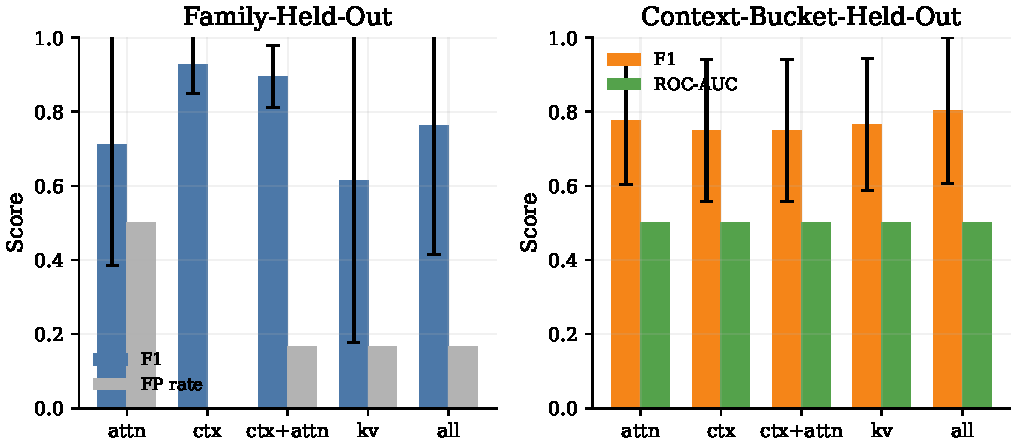
\includegraphics[width=0.95\linewidth]{figures/final_figures/paper_decision_signal_study.pdf}
    \caption{Held-out decision-signal study for workload-level positive-regime detection. Attention-only cues over-predict positive regimes, context is the strongest coarse predictor in the current setup, and all-feature detectors modestly improve context-bucket-held-out detection.}
    \label{fig:decision-signal-study}
\end{figure}

\subsection{Policy Case Study}

The policy results still matter, but they should be read as a focused case study rather than as proof of a universally best scheduler. A static attention heuristic is directionally useful, but it remains too permissive. The generic realistic policy \texttt{adaptive\_feature} is safer overall, but it misses several early-positive cases such as \texttt{Qwen3 @ ctx256}, \texttt{SmolLM2 @ ctx256}, and \texttt{Phi-3.5 @ ctx256}.

The more defensible message is that explicit KV-aware features can matter on some early-positive families. \texttt{kv\_regime} recovers \texttt{Qwen3 @ ctx256}, \texttt{SmolLM2 @ ctx256}, and \texttt{Phi-3.5 @ ctx256} without relying on oracle-like cost-model internals, but it is not uniformly dominant on every boundary point. We therefore frame this result as an existence proof that KV-aware decision features can be useful, not as a final scheduler contribution.

\begin{figure}[t]
    \centering
    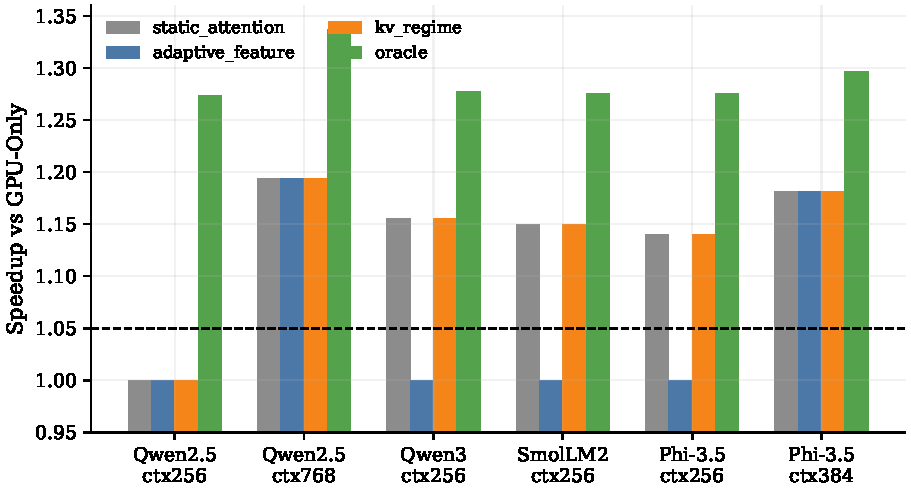
\includegraphics[width=0.95\linewidth]{figures/final_figures/paper_policy_comparison.pdf}
    \caption{Focused policy case study on selected early-positive workloads. KV-aware decision features can recover some early-positive cases that a generic realistic policy misses, but the figure should not be read as a universal ranking over all workloads.}
    \label{fig:policy-comparison}
\end{figure}

The policy comparison makes the paper's systems implication more concrete. Static attention offloading is often useful, but it does not capture why early-positive modern families differ from delayed-onset ones. The generic realistic policy \texttt{adaptive\_feature} is safer overall, but it still misses important early-positive points. In contrast, \texttt{kv\_regime} recovers several of these cases using only runtime-style KV-related signals and without direct oracle-like cost-model internals.

\subsection{Batch and Robustness Are Defensive Evidence}

The controlled batch study shows that batch is weaker than context in our current setup. On \texttt{Qwen2.5-1.5B}, online speedup remains exactly $1.000\times$ across $bs \in \{1,2,4,8\}$ at context 256, while remaining positive but nearly flat ($1.186\times$ to $1.194\times$) across the same batch sweep at context 768. Batch therefore changes magnitude within a regime more than it changes the regime itself.

The cost-model sensitivity analysis serves as a robustness check. Conservative, default, and optimistic virtual-PIM presets change absolute speedup numbers, but the canonical weak cases remain weak and the canonical long-context positive cases remain positive. Early-onset short-context points are closer to the decision boundary, but the main long-context story is stable. These results make the paper less vulnerable to the criticism that the conclusions are artifacts of a single narrow virtual backend setting.

\subsection{Summary of Experimental Takeaways}

Taken together, the experiments support four claims. First, virtual PIM value is regime-dependent rather than universal. Second, context length is the clearest coarse regime-entry variable in our current study. Third, the onset of positive offload value varies across model families. Fourth, KV-aware signals provide complementary predictive information near the boundary, while static attention labels alone are too permissive.
